%!TEX root = index.tex
%^^^^^^^^^^^^^^^^^^^^^^^^^^^
% make this the first line of all documents that are \include'd

% warn about incorrect/obsolete latex (yes, this goes before \documentclass)
\RequirePackage[l2tabu, orthodox, experimental]{nag}
% \PassOptionsToPackage{pdfpagelabels=false}{hyperref}
\documentclass{sig-alternate}

\usepackage[utf8]{inputenc}
\usepackage[english]{babel}

% you need to install 0.3 or newer of https://github.com/moewew/biblatex-trad
% in order to use trad-abbrv below:
\usepackage[backend=biber, style=trad-abbrv, giveninits=true, maxnames=99]{biblatex}
% this is necessary for weird error in bib
\usepackage[textsize=tiny]{todonotes}
\usepackage[
  pass,% keep layout unchanged
  % showframe,% show the layout
]{geometry}

\usepackage{microtype}
\usepackage{newtxtext}
\usepackage{url}
\usepackage{graphicx}
\usepackage{siunitx}
\usepackage{amsmath}
\usepackage{bookmark}
\usepackage{xcolor}
\usepackage[nolist]{acronym}
\usepackage{subcaption}
\usepackage{tabularx}
% \usepackage{tabulary}
\usepackage{enumitem}
\usepackage{multirow}
\usepackage{listings}
\usepackage{xspace}
\usepackage{comment}
% \usepackage{acmcopyright}
\usepackage{booktabs}

% let us use normal quotes and make them pretty
\usepackage[autostyle=true,english=american]{csquotes}
% \MakeOuterQuote{"}

% try harder to prevent widows and orphans
\widowpenalty=10000
\clubpenalty=10000

% fix hpyhenation of these words
\hyphenation{NetFPGA}

% make captions bold with subcaption
%\captionsetup{labelfont={bf}, textfont={bf}, singlelinecheck=off, justification=centering}
\captionsetup{labelfont={bf}, textfont={bf}, singlelinecheck=off}

% set up siunitx
\sisetup{detect-all=true, binary-units, free-standing-units, range-units=single}

% don't use typewriter font for URLs
\urlstyle{same}

% prefixes for \autoref
\AtBeginDocument{
\renewcommand{\sectionautorefname}{Section}
\renewcommand{\subsectionautorefname}{Section}
\renewcommand{\subsectionautorefname}{Section}
}

% highlight missing references and citations with red background
\makeatletter
\patchcmd{\@setref}{\bfseries??}{\colorbox{red!30}{\detokenize{#3}}}{}{}
\def\abx@missing#1{\colorbox{red!30}{\detokenize{#1}}}
\makeatother

% the bibliography is here
\addbibresource{index.bib}

% transmogrify the bibliography:
% 1. don't show various fields such as ISBNs, etc.
\AtEveryBibitem{\clearfield{isbn}}
\AtEveryBibitem{\clearfield{issn}}
\AtEveryBibitem{\clearlist{institution}}
\AtEveryBibitem{\clearfield{doi}}
% \AtEveryBibitem{\clearfield{url}}
\AtEveryBibitem{\clearlist{publisher}}
% \AtEveryBibitem{\clearlist{location}}
\AtEveryBibitem{\clearfield{series}}
\AtEveryBibitem{\clearfield{note}}
% \AtEveryBibitem{\clearfield{pages}}
\AtEveryBibitem{\clearfield{pagetotal}}
\AtEveryBibitem{\clearfield{volume}}
\AtEveryBibitem{
        \ifboolexpr{test {\ifentrytype{article}}}{\clearfield{number}}{}
        \ifboolexpr{not test {\ifentrytype{misc}}}{\clearfield{url}}{}
}
% 2. other transforms
\DeclareSourcemap{
        \maps[datatype=bibtex]{
                \map{
                        % shorten conferences
                        \step[fieldsource=booktitle,
                                match={.*Internet Measurement Conference.*},
                                replace={Proc. ACM IMC}]
                        \step[fieldsource=booktitle,
                                match={.*Networked Systems Design and Implementation.*},
                                replace={Proc. USENIX NSDI}]
                        \step[fieldsource=booktitle,
                                match={.*Hot Topics in Networks.*},
                                replace={Proc. ACM HotNets}]
                        \step[fieldsource=booktitle,
                                match={.*Operating Systems Design and Implementation.*},
                                replace={Proc. USENIX OSDI}]
                        \step[fieldsource=booktitle,
                                match={.*USENIX Annual Technical Conference.*},
                                replace={Proc. USENIX ATC}]
                        \step[fieldsource=booktitle,
                                match={.*USENIX Conference on File and Storage Technologies.*},
                                replace={Proc. USENIX FAST}]
                        \step[fieldsource=booktitle,
                                match={.*European Conference on Computer Systems.*},
                                replace={Proc. ACM EuroSys}]
                        \step[fieldsource=booktitle,
                                match={.*Symposium on Operating Systems Principles.*},
                                replace={Proc. ACM SOSP}]
                        \step[fieldsource=booktitle,
                                match={.*(USENIX Security Symposium|USENIX Conference on Security).*},
                                replace={Proc. USENIX Security}]
                        \step[fieldsource=booktitle,
                                match={.*USENIX Symposium on Internet Technologies and Systems.*},
                                replace={Proc. USENIX USITS}]
                        \step[fieldsource=booktitle,
                                match={.*Emerging Networking E.periments and Technologies.*},
                                replace={Proc. ACM CoNEXT}]
                        \step[fieldsource=booktitle,
                                match={.*INFOCOM.*},
                                replace={Proc. IEEE Infocom}]
                        \step[fieldsource=booktitle,
                                match={.*Roedunet.*},
                                replace={Proc. IEEE RoEduNet}]
                        \step[fieldsource=booktitle,
                                match={.*Architectural Support for Programming Languages and Operating Systems.*},
                                replace={Proc. ACM ASPLOS}]
                        \step[fieldsource=booktitle,
                                match={.*Symposium on Software Defined Networking Research.*},
                                replace={Proc. ACM SOSR}]
                        \step[fieldsource=booktitle,
                                match={.*Architectures? for Networking and Communications Systems.*},
                                replace={Proc. ACM ANCS}]
                        \step[fieldsource=booktitle,
                                match={.*SIGMOD International Conference on Management of Data.*},
                                replace={Proc. ACM SIGMOD}]
                        % keep this last
                        \step[fieldsource=booktitle,
                                match={.*(SIGCOMM|Special Interest Group on Data Communication|Applications, Technologies, Architectures, and Protocols|Communications Architectures and Protocols).*},
                                replace={Proc. ACM SIGCOMM}]
                        % shorten journals
                        \step[fieldsource=journal,
                                match={.*IEEE Journal on Selected Areas in Communication.*},
                                replace={IEEE JSAC}]
                        \step[fieldsource=journal,
                                match={.*Comput. Commun. Rev..*},
                                replace={ACM SIGCOMM CCR}]
                }
        }
}
% 3. skip the "In:" for @inproceedings and change some month abbreviations
% 3. skip the "In:" for @inproceedings and change some month abbreviations
\DefineBibliographyStrings{english}{
        in               = {},
        page             = {p\adddot},
        pages            = {pp\adddot},
        june             = {Jun\adddot},
        july             = {Jul\adddot},
        september        = {Sep\adddot},
}

\hypersetup{pdffitwindow=true,pdfpagelayout=SinglePage,pdfpagemode=UseThumbs}

\setlength\paperheight{11in}
\setlength\paperwidth{8.5in}
\setlength{\textwidth}{7in}
\setlength{\textheight}{9.25in}
\setlength{\oddsidemargin}{-.25in}
\setlength{\evensidemargin}{-.25in}

\begin{document}
\begin{acronym}
  \acro{SDN}{Software Defined Networks}
\end{acronym}



\title{Munich Internet Research Retreat 2016}

\numberofauthors{1}
\author{
\begin{tabular*}{0.50\textwidth}%
{@{\extracolsep{50pt}}cc}
Georg Carle & Lars Eggert \\
\affaddr{TU Munich} & \affaddr{NetApp} \\
%\affaddr{Munich, DE} & \affaddr{Munich, DE} \\
\email{carle@in.tum.de} & \email{lars@netapp.com}
\end{tabular*}\\
\begin{tabular}{c}
\end{tabular}\\
\begin{tabular*}{0.60\textwidth}%
{@{\extracolsep{35pt}}cc}
Wolfgang Kellerer & Jörg Ott \\
\affaddr{TU Munich} & \affaddr{TU Munich} \\
%\affaddr{Munich, DE} & \affaddr{Munich, DE} \\
\email{wolfgang.kellerer@tum.de} & \email{ott@in.tum.de}
\end{tabular*}\\
\begin{tabular}{c}
\end{tabular}\\
\begin{tabular}{c}
{\normalsize This article is an editorial note submitted to CCR. It has NOT
been peer reviewed.}\\
{\normalsize The authors take full responsibility for this article's
technical content. Comments can be posted through CCR Online.}
\end{tabular}
}

\maketitle

\begin{abstract}

This article summarises a 2 day long Munich Internet Research Retreat held in
November 2016.  The goal of the retreat was to provide a forum for both
academic and industrial researchers to exchange ideas and get feedback on
their current work. It was organized in a spirit that is similar to an highly
interactive Dagstuhl seminars, with a very limited number of full-length
talks, while dedicating most of the time to poster sessions, panels and group
discussions. The entire set of presentations delivered during the seminar is
made publicly available at \cite{mir-materials}.

\end{abstract}

% referrred: http://www.acm.org/about/class/ccs98-html
%\category{C.2.3}{Computer-Communication Networks}{Network Operations}[Network
%monitoring]

% referred: http://www.acm.org/sigs/publications/sigguide-v2.2sp
%\terms{Measurement, Performance}

%\keywords{SDN, NFV, Security, IoT, Internet measurements}

% sections
%----------------------------------------------------------------------
%**************************************************************************
\section{Introduction}\label{sec:introduction}
%**************************************************************************

%------------------------ Motivation
%------------------------ Goals
\todo[inline]{Motivation and Goals}

%**************************************************************************
\section{Invited Presentations}\label{sec:invited-presentations}
%**************************************************************************

The invited presentations were intended as a basis for triggering discussions
and identifying areas for group work.

% ------------ Dirk Kutscher
\subsection{Edge Computing considered harmful}


% ------------ Alexander von Gemler
\subsection{Towards A Clean Slate -- Digital Sovereignty in the Post Snowden Era}


% ------------ Artur Hecker
\subsection{On software network management}


% ------------ Wolfgang Kellerer
\subsection{FlexNets: Quantifying Flexibility in Communication Networks}


% ------------ Brian Trammell
\subsection{An Accidental Internet Architecture}


% ------------ Vaibhav Bajpai
\subsection{Measuring IPv6 Performance}


% ------------ Minoo Ruohi
\subsection{Path tracing and validation of IPv4 and IPv6 siblings}


% ------------ Laurent Vanbever
\subsection{SWIFT: Predictive Fast Reroute upon Remote BGP Disruptions}


% ------------ Christian Prehofer
\subsection{Open Platforms for Cyber-physical systems}


% ------------ Holger Kinkelin
\subsection{Collaborative intrusion handling using the Blackboard-Pattern}



%**************************************************************************
\section{Parallel Group Work}\label{sec:parallel-group-work}
%**************************************************************************

The afternoon sessions were used to discuss certain topics in more depth in
smaller groups. This section summarises the discussions of each group.

% ------------- Andreas Blenk (TUM LKN)
\subsection{SDN/NFV Measurements}

% ------------- Georg Carle
\subsection{SDN++: Applications Perspective}

The breakout session entitled SDN++ dealt with SDN from the perspective of how to apply SDN, and how to introduce improvements to SDN (thereby creating SDN++), for better meeting the identified requirements.
Participants of the breakout session were Laurent Vanbevier, Artur Hecker, Wolfgang Kellerer, Edwin Cordeiro and Georg Carle, the latter also being the presenter of the results.
The method of the working group was first to identify relevant application areas of SDN, then assess to which extent known SDN approaches have shortcomings (i.e., identifying the `SDN pain areas`), and subsequently identifying promising approaches for improving SDN.
The application areas of SDN were (1) establishing means for programmability of the network, which can be used for improving certain network properties, (2) management of advanced cellular networks, in particular 5G networks, for different capabilities such as network slicing, and (3) providing means to add sophisticated control functionality to corporate networks, such as adding flexible access control. 
Identified weaknesses of existing SDN were the fact that existing SDN southbound interfaces, in particular OpenFlow, operate on a low level of abstraction, which makes programming of the network time-consuming and error prone. 
Identified areas of improvement and need for further work were specifying suitable high-level interfaces and abstractions.
There further is the need to develop tools that are capable of automatically translate high-level specifications to low-level configuration. A complete tool chain is required.
This includes measurement tools that are capable of monitoring changes. Network programmability is beneficial for measurement tools.
It is expected that SDN management tools will facilitate to deal with the programmability of networks.
Furthermore, verification tools will allow to detect and prevent attempts of wrongly programming the network.    
These tools will form a network operating system, with tools that operate on top of the operating system functions.
Another need for improvement is the development of a clear transition path from today's networks to future SDN-based networks. This includes to identify which legacy functionalities from today's networks we assume being able to depend on in SDN deployments.
           



% ------------- Lars Eggert
\subsection{QUIC}

% Do you need to be Google or a large CDN deploy a protocol. Repeated failure of good ideas (HIP and SCTP). Only if two endpoints can do something and not require middleware to make changes is easier to deploy. Brian mentioned that QUIC works because controls both endpoints (browser and servers) and also pointed to TSV area slides.


% ------------- Johannes Naab / Heiko Niedermayer
\subsection{DDoS Defence beyond Centralization}

% ------------- Alexander von Gernler
\subsection{Security}

% ------------- Aaron
\subsection{IoT}
%**************************************************************************
\section{Posters}\label{sec:posters}
%**************************************************************************

Participants were also encouraged to volunteer to bring a poster to provide a
perspective into their recent measurement research work.

\subsection{The cost of Security in the SDN control Plane}

In OpenFlow enabled Software Defined Networks (SDNs) network control is
carried out remotely via a control connection. In order to deploy OpenFlow in
production networks, security of the control connection is crucial. For
OpenFlow connections TLS encryption is recommended by the specification. In
this work, we analyze the TLS support in the OpenFlow eco-system. In
particular, we implemented a performance measurement tool for encrypted
OpenFlow connections, as there is non available.  Our first results show that
security comes at an extra cost and hence further work is needed to design
efficient mechanisms taking the security-delay trade-off into account.

Published: R. Durner, W. Kellerer, The cost of Security in the SDN control
Plane, ACM CoNEXT 2015 - Student Workshop, Heidelberg, Germany, Dezember 2015.

% -------- Renata
%\subsection{HostView}

%**************************************************************************
\section{Conclusions and Next Steps}\label{sec:conclusion}
%**************************************************************************

%**************************************************************************
\subsection*{Acknowledgements}\label{sec:acknowledgement}
%**************************************************************************

This seminar was located at the TUM Science and Study Center in Raitenhaslach,
Germany, supported by by NetApp, Huawei, and TUM.  The organisers would like
to thank the participants (alphabetically ordered by first name) for their
contributions $-$

\begin{figure}[t!]
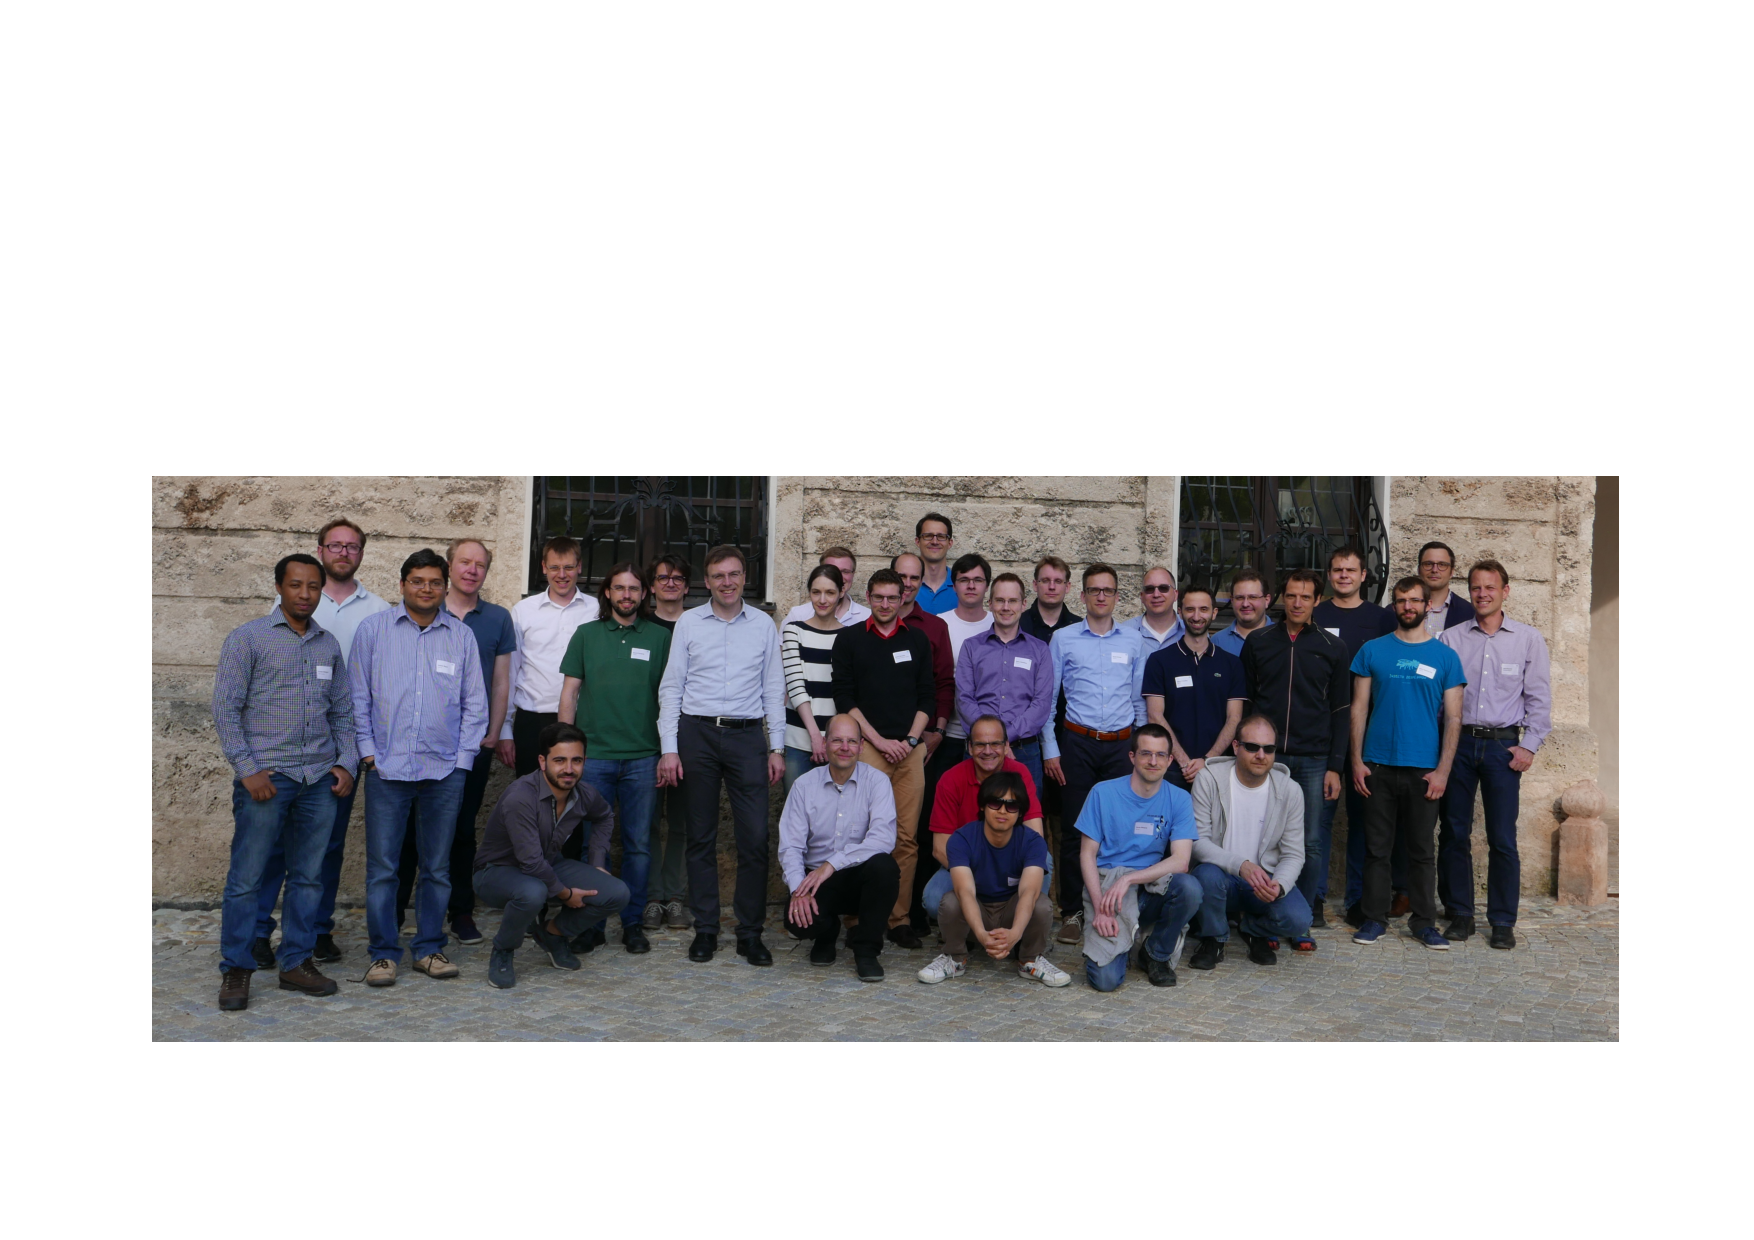
\includegraphics[width=1.0\linewidth]{figures/group-photo}
\end{figure}

\href{}{Aaron Yi Ding} (TUM CM),
\href{}{Alberto Martínez Alba} (TUM LKN),
\href{}{Alexander von Gernler} (genua GmbH),
\href{}{Andreas Blenk} (TUM LKN),
\href{}{Arsany Basta} (TUM LKN),
\href{}{Artur Hecker} (Huawei),
\href{}{Brian Trammell} (ETH Zürich),
\href{}{Christian Prehofer} (fortiss, TUM),
\href{}{Claas Lorenz} (genua GmbH),
\href{}{Daniel Raumer} (TUM NET),
\href{}{Dirk Kutscher} (Huawei),
\href{}{Edwin Cordeiro} (TUM NET),
\href{}{Florian Westphal} (Red Hat),
\href{}{Georg Carle} (TUM NET),
\href{}{Hagen Paul Pfeifer} (Rohde \& Schwarz),
\href{}{Heiko Niedermayer} (TUM NET),
\href{}{Johannes Naab} (TUM NET),
\href{}{Jörg Ott} (TUM CM),
\href{}{Holger Kinkelin} (TUM NET),
\href{}{Lars Eggert} (NetApp),
\href{}{Laurent Vanbever} (ETH Zürich),
\href{}{Marco Hoffmann} (Nokia Bell Labs),
\href{}{Markus Klügel} (TUM LKN),
\href{}{Matthias Wachs} (TUM NET),
\href{}{Minoo Rouhi} (TUM NET),
\href{}{Mirja Kühlewind} (ETH Zurich),
\href{}{Nemanja Djeric} (TUM LKN),
\href{}{Paul Emmerich} (TUM NET),
\href{}{Pavel Laskov} (Huawei),
\href{}{Peter Babarczi} (TUM NET),
\href{}{Raphael Durner} (TUM LKN),
\href{}{Rastin Pries} (Nokia Bell Labs),
\href{}{Rolf Winter} (University of Applied Sciences Augsburg),
\href{}{Sebastian Gallenmüller} (TUM NET),
\href{}{Vaibhav Bajpai} (Jacobs University Bremen),
\href{}{Wolfgang Kellerer} (TUM LKN),


%----------------------------------------------------------------------

% bibliography

%\AtNextBibliography{\small}
\setlength\bibitemsep{2pt}
\printbibliography[title=REFERENCES, heading=bibnumbered]

\end{document}
